\documentclass[1p]{elsarticle_modified}
%\bibliographystyle{elsarticle-num}

%\usepackage[colorlinks]{hyperref}
%\usepackage{abbrmath_seonhwa} %\Abb, \Ascr, \Acal ,\Abf, \Afrak
\usepackage{amsfonts}
\usepackage{amssymb}
\usepackage{amsmath}
\usepackage{amsthm}
\usepackage{scalefnt}
\usepackage{amsbsy}
\usepackage{kotex}
\usepackage{caption}
\usepackage{subfig}
\usepackage{color}
\usepackage{graphicx}
\usepackage{xcolor} %% white, black, red, green, blue, cyan, magenta, yellow
\usepackage{float}
\usepackage{setspace}
\usepackage{hyperref}

\usepackage{tikz}
\usetikzlibrary{arrows}

\usepackage{multirow}
\usepackage{array} % fixed length table
\usepackage{hhline}

%%%%%%%%%%%%%%%%%%%%%
\makeatletter
\renewcommand*\env@matrix[1][\arraystretch]{%
	\edef\arraystretch{#1}%
	\hskip -\arraycolsep
	\let\@ifnextchar\new@ifnextchar
	\array{*\c@MaxMatrixCols c}}
\makeatother %https://tex.stackexchange.com/questions/14071/how-can-i-increase-the-line-spacing-in-a-matrix
%%%%%%%%%%%%%%%

\usepackage[normalem]{ulem}

\newcommand{\msout}[1]{\ifmmode\text{\sout{\ensuremath{#1}}}\else\sout{#1}\fi}
%SOURCE: \msout is \stkout macro in https://tex.stackexchange.com/questions/20609/strikeout-in-math-mode

\newcommand{\cancel}[1]{
	\ifmmode
	{\color{red}\msout{#1}}
	\else
	{\color{red}\sout{#1}}
	\fi
}

\newcommand{\add}[1]{
	{\color{blue}\uwave{#1}}
}

\newcommand{\replace}[2]{
	\ifmmode
	{\color{red}\msout{#1}}{\color{blue}\uwave{#2}}
	\else
	{\color{red}\sout{#1}}{\color{blue}\uwave{#2}}
	\fi
}

\newcommand{\Sol}{\mathcal{S}} %segment
\newcommand{\D}{D} %diagram
\newcommand{\A}{\mathcal{A}} %arc


%%%%%%%%%%%%%%%%%%%%%%%%%%%%%5 test

\def\sl{\operatorname{\textup{SL}}(2,\Cbb)}
\def\psl{\operatorname{\textup{PSL}}(2,\Cbb)}
\def\quan{\mkern 1mu \triangleright \mkern 1mu}

\theoremstyle{definition}
\newtheorem{thm}{Theorem}[section]
\newtheorem{prop}[thm]{Proposition}
\newtheorem{lem}[thm]{Lemma}
\newtheorem{ques}[thm]{Question}
\newtheorem{cor}[thm]{Corollary}
\newtheorem{defn}[thm]{Definition}
\newtheorem{exam}[thm]{Example}
\newtheorem{rmk}[thm]{Remark}
\newtheorem{alg}[thm]{Algorithm}

\newcommand{\I}{\sqrt{-1}}
\begin{document}

%\begin{frontmatter}
%
%\title{Boundary parabolic representations of knots up to 8 crossings}
%
%%% Group authors per affiliation:
%\author{Yunhi Cho} 
%\address{Department of Mathematics, University of Seoul, Seoul, Korea}
%\ead{yhcho@uos.ac.kr}
%
%
%\author{Seonhwa Kim} %\fnref{s_kim}}
%\address{Center for Geometry and Physics, Institute for Basic Science, Pohang, 37673, Korea}
%\ead{ryeona17@ibs.re.kr}
%
%\author{Hyuk Kim}
%\address{Department of Mathematical Sciences, Seoul National University, Seoul 08826, Korea}
%\ead{hyukkim@snu.ac.kr}
%
%\author{Seokbeom Yoon}
%\address{Department of Mathematical Sciences, Seoul National University, Seoul, 08826,  Korea}
%\ead{sbyoon15@snu.ac.kr}
%
%\begin{abstract}
%We find all boundary parabolic representation of knots up to 8 crossings.
%
%\end{abstract}
%\begin{keyword}
%    \MSC[2010] 57M25 
%\end{keyword}
%
%\end{frontmatter}

%\linenumbers
%\tableofcontents
%
\newcommand\colored[1]{\textcolor{white}{\rule[-0.35ex]{0.8em}{1.4ex}}\kern-0.8em\color{red} #1}%
%\newcommand\colored[1]{\textcolor{white}{ #1}\kern-2.17ex	\textcolor{white}{ #1}\kern-1.81ex	\textcolor{white}{ #1}\kern-2.15ex\color{red}#1	}

{\Large $\underline{12n_{0819}~(K12n_{0819})}$}

\setlength{\tabcolsep}{10pt}
\renewcommand{\arraystretch}{1.6}
\vspace{1cm}\begin{tabular}{m{100pt}>{\centering\arraybackslash}m{274pt}}
\multirow{5}{120pt}{
	\centering
	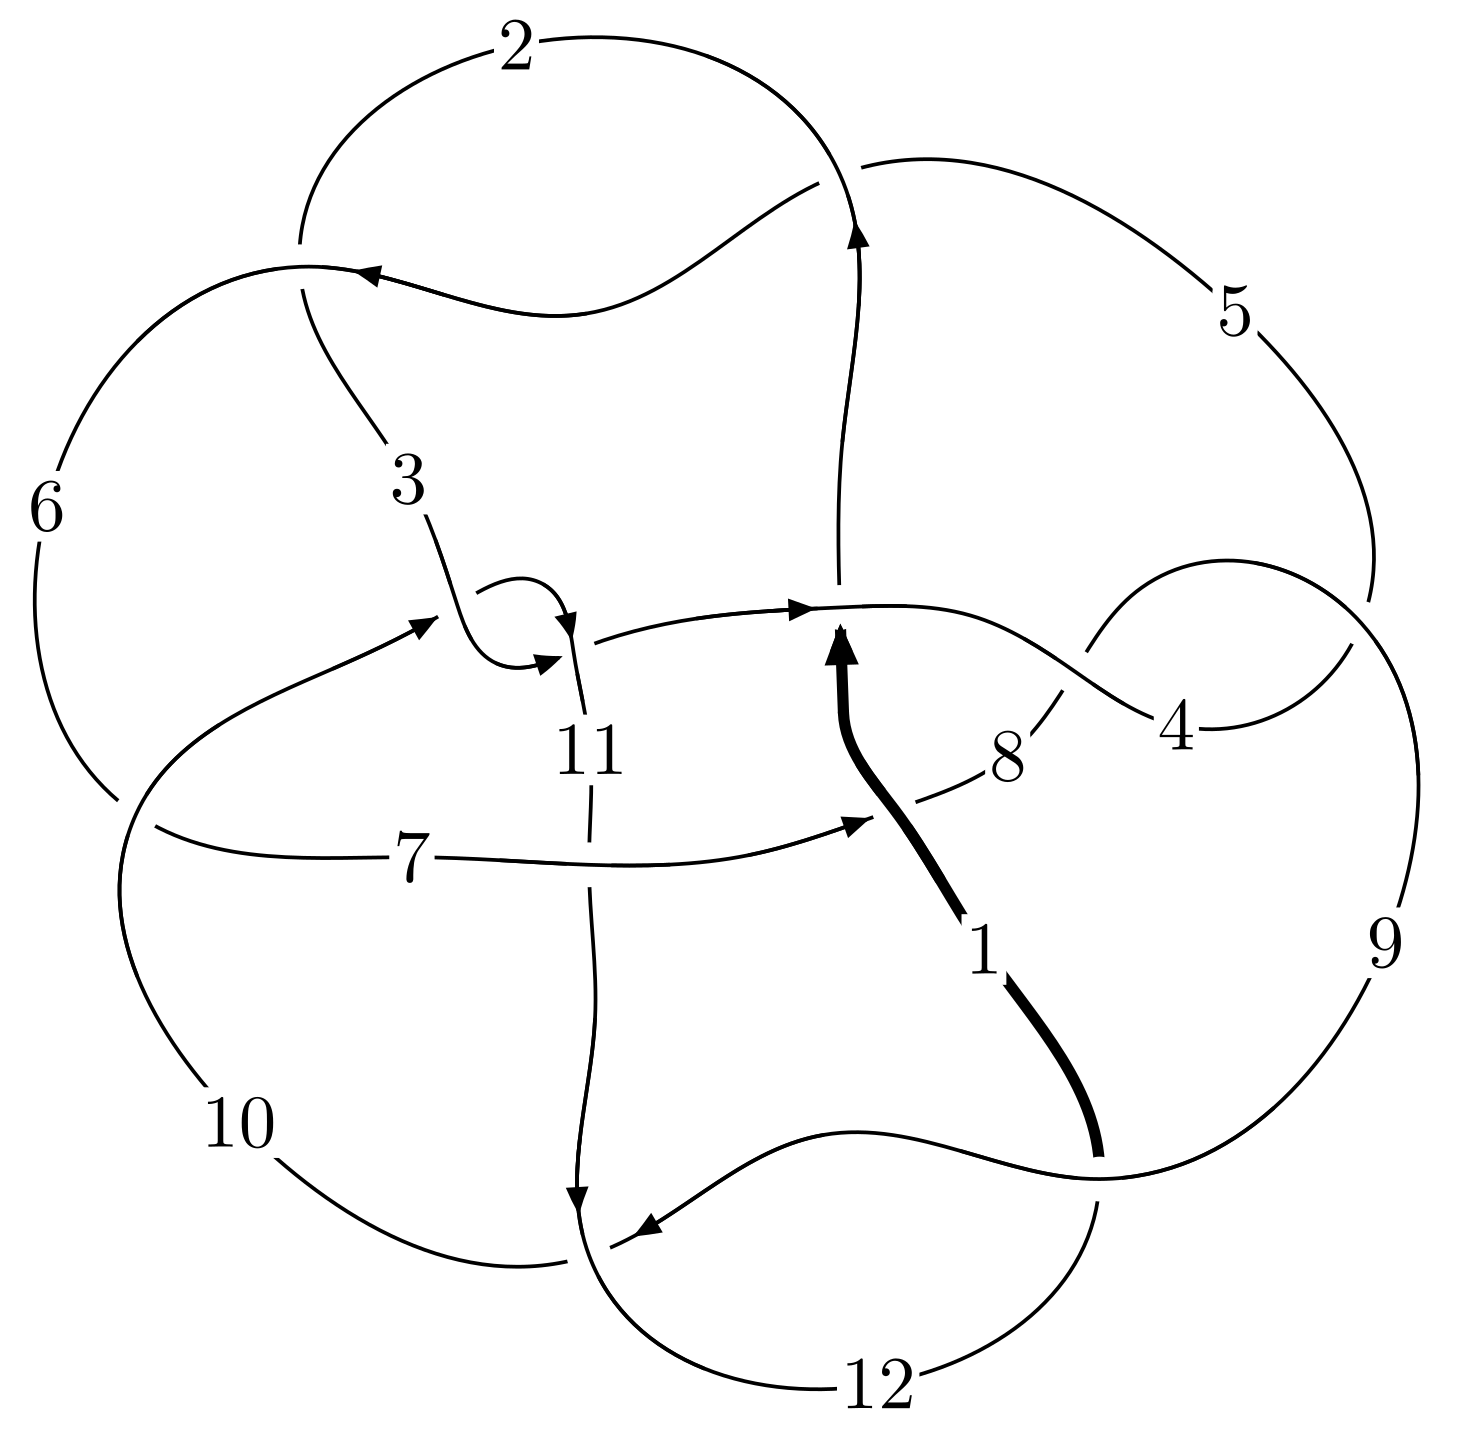
\includegraphics[width=112pt]{../../../GIT/diagram.site/Diagrams/png/2908_12n_0819.png}\\
\ \ \ A knot diagram\footnotemark}&
\allowdisplaybreaks
\textbf{Linearized knot diagam} \\
\cline{2-2}
 &
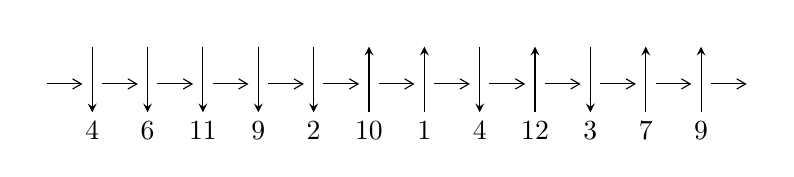
\begin{tikzpicture}[x=20pt, y=17pt]
	% nodes
	\node (C0) at (0, 0) {};
	\node (C1) at (1, 0) {};
	\node (C1U) at (1, +1) {};
	\node (C1D) at (1, -1) {4};

	\node (C2) at (2, 0) {};
	\node (C2U) at (2, +1) {};
	\node (C2D) at (2, -1) {6};

	\node (C3) at (3, 0) {};
	\node (C3U) at (3, +1) {};
	\node (C3D) at (3, -1) {11};

	\node (C4) at (4, 0) {};
	\node (C4U) at (4, +1) {};
	\node (C4D) at (4, -1) {9};

	\node (C5) at (5, 0) {};
	\node (C5U) at (5, +1) {};
	\node (C5D) at (5, -1) {2};

	\node (C6) at (6, 0) {};
	\node (C6U) at (6, +1) {};
	\node (C6D) at (6, -1) {10};

	\node (C7) at (7, 0) {};
	\node (C7U) at (7, +1) {};
	\node (C7D) at (7, -1) {1};

	\node (C8) at (8, 0) {};
	\node (C8U) at (8, +1) {};
	\node (C8D) at (8, -1) {4};

	\node (C9) at (9, 0) {};
	\node (C9U) at (9, +1) {};
	\node (C9D) at (9, -1) {12};

	\node (C10) at (10, 0) {};
	\node (C10U) at (10, +1) {};
	\node (C10D) at (10, -1) {3};

	\node (C11) at (11, 0) {};
	\node (C11U) at (11, +1) {};
	\node (C11D) at (11, -1) {7};

	\node (C12) at (12, 0) {};
	\node (C12U) at (12, +1) {};
	\node (C12D) at (12, -1) {9};
	\node (C13) at (13, 0) {};

	% arrows
	\draw[->,>={angle 60}]
	(C0) edge (C1) (C1) edge (C2) (C2) edge (C3) (C3) edge (C4) (C4) edge (C5) (C5) edge (C6) (C6) edge (C7) (C7) edge (C8) (C8) edge (C9) (C9) edge (C10) (C10) edge (C11) (C11) edge (C12) (C12) edge (C13) ;	\draw[->,>=stealth]
	(C1U) edge (C1D) (C2U) edge (C2D) (C3U) edge (C3D) (C4U) edge (C4D) (C5U) edge (C5D) (C6D) edge (C6U) (C7D) edge (C7U) (C8U) edge (C8D) (C9D) edge (C9U) (C10U) edge (C10D) (C11D) edge (C11U) (C12D) edge (C12U) ;
	\end{tikzpicture} \\
\hhline{~~} \\& 
\textbf{Solving Sequence} \\ \cline{2-2} 
 &
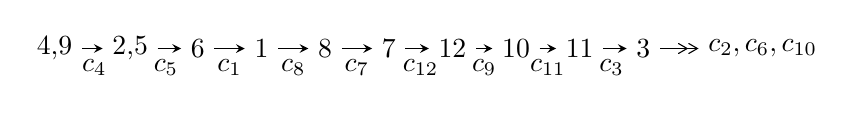
\begin{tikzpicture}[x=23pt, y=7pt]
	% node
	\node (A0) at (-1/8, 0) {4,9};
	\node (A1) at (17/16, 0) {2,5};
	\node (A2) at (17/8, 0) {6};
	\node (A3) at (25/8, 0) {1};
	\node (A4) at (33/8, 0) {8};
	\node (A5) at (41/8, 0) {7};
	\node (A6) at (49/8, 0) {12};
	\node (A7) at (57/8, 0) {10};
	\node (A8) at (65/8, 0) {11};
	\node (A9) at (73/8, 0) {3};
	\node (C1) at (1/2, -1) {$c_{4}$};
	\node (C2) at (13/8, -1) {$c_{5}$};
	\node (C3) at (21/8, -1) {$c_{1}$};
	\node (C4) at (29/8, -1) {$c_{8}$};
	\node (C5) at (37/8, -1) {$c_{7}$};
	\node (C6) at (45/8, -1) {$c_{12}$};
	\node (C7) at (53/8, -1) {$c_{9}$};
	\node (C8) at (61/8, -1) {$c_{11}$};
	\node (C9) at (69/8, -1) {$c_{3}$};
	\node (A10) at (11, 0) {$c_{2},c_{6},c_{10}$};

	% edge
	\draw[->,>=stealth]	
	(A0) edge (A1) (A1) edge (A2) (A2) edge (A3) (A3) edge (A4) (A4) edge (A5) (A5) edge (A6) (A6) edge (A7) (A7) edge (A8) (A8) edge (A9) ;
	\draw[->>,>={angle 60}]	
	(A9) edge (A10);
\end{tikzpicture} \\ 

\end{tabular} \\

\footnotetext{
The image of knot diagram is generated by the software ``\textbf{Draw programme}" developed by Andrew Bartholomew(\url{http://www.layer8.co.uk/maths/draw/index.htm\#Running-draw}), where we modified some parts for our purpose(\url{https://github.com/CATsTAILs/LinksPainter}).
}\phantom \\ \newline 
\centering \textbf{Ideals for irreducible components\footnotemark of $X_{\text{par}}$} 
 
\begin{align*}
I^u_{1}&=\langle 
8.73090\times10^{293} u^{77}-3.56351\times10^{294} u^{76}+\cdots+7.84651\times10^{296} b-4.65322\times10^{297},\\
\phantom{I^u_{1}}&\phantom{= \langle  }-1.85338\times10^{298} u^{77}+6.45142\times10^{298} u^{76}+\cdots+4.37678\times10^{300} a+6.50906\times10^{300},\\
\phantom{I^u_{1}}&\phantom{= \langle  }u^{78}-4 u^{77}+\cdots-34268 u+2789\rangle \\
I^u_{2}&=\langle 
976963699145 u^{24}-5356482432121 u^{23}+\cdots+6473712830526 b+4457277781243,\\
\phantom{I^u_{2}}&\phantom{= \langle  }-4338891421343 u^{24}+18419785693814 u^{23}+\cdots+12947425661052 a-28103666444157,\\
\phantom{I^u_{2}}&\phantom{= \langle  }u^{25}-5 u^{24}+\cdots+3 u-1\rangle \\
\\
\end{align*}
\raggedright * 2 irreducible components of $\dim_{\mathbb{C}}=0$, with total 103 representations.\\
\footnotetext{All coefficients of polynomials are rational numbers. But the coefficients are sometimes approximated in decimal forms when there is not enough margin.}
\newpage
\renewcommand{\arraystretch}{1}
\centering \section*{I. $I^u_{1}= \langle 8.73\times10^{293} u^{77}-3.56\times10^{294} u^{76}+\cdots+7.85\times10^{296} b-4.65\times10^{297},\;-1.85\times10^{298} u^{77}+6.45\times10^{298} u^{76}+\cdots+4.38\times10^{300} a+6.51\times10^{300},\;u^{78}-4 u^{77}+\cdots-34268 u+2789 \rangle$}
\flushleft \textbf{(i) Arc colorings}\\
\begin{tabular}{m{7pt} m{180pt} m{7pt} m{180pt} }
\flushright $a_{4}=$&$\begin{pmatrix}1\\0\end{pmatrix}$ \\
\flushright $a_{9}=$&$\begin{pmatrix}0\\u\end{pmatrix}$ \\
\flushright $a_{2}=$&$\begin{pmatrix}0.00423457 u^{77}-0.0147401 u^{76}+\cdots+47.3144 u-1.48718\\-0.00111271 u^{77}+0.00454153 u^{76}+\cdots-68.9860 u+5.93031\end{pmatrix}$ \\
\flushright $a_{5}=$&$\begin{pmatrix}1\\u^2\end{pmatrix}$ \\
\flushright $a_{6}=$&$\begin{pmatrix}0.00437670 u^{77}-0.0163847 u^{76}+\cdots+19.7784 u-1.75814\\-0.00313818 u^{77}+0.0102642 u^{76}+\cdots+84.8849 u-8.41119\end{pmatrix}$ \\
\flushright $a_{1}=$&$\begin{pmatrix}0.00312185 u^{77}-0.0101986 u^{76}+\cdots-21.6716 u+4.44313\\-0.00111271 u^{77}+0.00454153 u^{76}+\cdots-68.9860 u+5.93031\end{pmatrix}$ \\
\flushright $a_{8}=$&$\begin{pmatrix}u\\u\end{pmatrix}$ \\
\flushright $a_{7}=$&$\begin{pmatrix}-0.00192164 u^{77}+0.0114186 u^{76}+\cdots-261.075 u+19.1357\\0.00123597 u^{77}-0.00425560 u^{76}+\cdots-33.1124 u+3.71756\end{pmatrix}$ \\
\flushright $a_{12}=$&$\begin{pmatrix}0.00312185 u^{77}-0.0101986 u^{76}+\cdots-21.6716 u+4.44313\\-0.00176996 u^{77}+0.00593289 u^{76}+\cdots+0.741219 u-0.453273\end{pmatrix}$ \\
\flushright $a_{10}=$&$\begin{pmatrix}-0.000969232 u^{77}+0.000832254 u^{76}+\cdots+160.099 u-12.1813\\-0.00313055 u^{77}+0.0146618 u^{76}+\cdots-202.608 u+15.4460\end{pmatrix}$ \\
\flushright $a_{11}=$&$\begin{pmatrix}-0.00124230 u^{77}+0.00728569 u^{76}+\cdots-177.510 u+17.3463\\0.00191628 u^{77}-0.00793871 u^{76}+\cdots+50.3738 u-5.09448\end{pmatrix}$ \\
\flushright $a_{3}=$&$\begin{pmatrix}-0.00105957 u^{77}+0.00386563 u^{76}+\cdots-11.5396 u+5.70652\\0.00156637 u^{77}-0.00526645 u^{76}+\cdots-25.0713 u+1.19390\end{pmatrix}$\\&\end{tabular}
\flushleft \textbf{(ii) Obstruction class $= -1$}\\~\\
\flushleft \textbf{(iii) Cusp Shapes $= 0.00717324 u^{77}-0.0329693 u^{76}+\cdots+172.137 u-9.92485$}\\~\\
\newpage\renewcommand{\arraystretch}{1}
\flushleft \textbf{(iv) u-Polynomials at the component}\newline \\
\begin{tabular}{m{50pt}|m{274pt}}
Crossings & \hspace{64pt}u-Polynomials at each crossing \\
\hline $$\begin{aligned}c_{1}\end{aligned}$$&$\begin{aligned}
&u^{78}-2 u^{77}+\cdots+5080 u-1808
\end{aligned}$\\
\hline $$\begin{aligned}c_{2},c_{5}\end{aligned}$$&$\begin{aligned}
&u^{78}+4 u^{77}+\cdots-177548 u-41707
\end{aligned}$\\
\hline $$\begin{aligned}c_{3},c_{10}\end{aligned}$$&$\begin{aligned}
&u^{78}- u^{77}+\cdots-7 u+85
\end{aligned}$\\
\hline $$\begin{aligned}c_{4},c_{8}\end{aligned}$$&$\begin{aligned}
&u^{78}+4 u^{77}+\cdots+34268 u+2789
\end{aligned}$\\
\hline $$\begin{aligned}c_{6}\end{aligned}$$&$\begin{aligned}
&u^{78}-6 u^{77}+\cdots-120616 u-6256
\end{aligned}$\\
\hline $$\begin{aligned}c_{7}\end{aligned}$$&$\begin{aligned}
&u^{78}-2 u^{77}+\cdots-35004 u-5048
\end{aligned}$\\
\hline $$\begin{aligned}c_{9},c_{12}\end{aligned}$$&$\begin{aligned}
&u^{78}+4 u^{77}+\cdots-21648 u-1747
\end{aligned}$\\
\hline $$\begin{aligned}c_{11}\end{aligned}$$&$\begin{aligned}
&u^{78}+2 u^{77}+\cdots+1038 u-463
\end{aligned}$\\
\hline
\end{tabular}\\~\\
\newpage\renewcommand{\arraystretch}{1}
\flushleft \textbf{(v) Riley Polynomials at the component}\newline \\
\begin{tabular}{m{50pt}|m{274pt}}
Crossings & \hspace{64pt}Riley Polynomials at each crossing \\
\hline $$\begin{aligned}c_{1}\end{aligned}$$&$\begin{aligned}
&y^{78}+86 y^{77}+\cdots+33365824 y+3268864
\end{aligned}$\\
\hline $$\begin{aligned}c_{2},c_{5}\end{aligned}$$&$\begin{aligned}
&y^{78}-54 y^{77}+\cdots-15298685406 y+1739473849
\end{aligned}$\\
\hline $$\begin{aligned}c_{3},c_{10}\end{aligned}$$&$\begin{aligned}
&y^{78}-51 y^{77}+\cdots-50879 y+7225
\end{aligned}$\\
\hline $$\begin{aligned}c_{4},c_{8}\end{aligned}$$&$\begin{aligned}
&y^{78}+74 y^{77}+\cdots+243548106 y+7778521
\end{aligned}$\\
\hline $$\begin{aligned}c_{6}\end{aligned}$$&$\begin{aligned}
&y^{78}+36 y^{77}+\cdots-7231852480 y+39137536
\end{aligned}$\\
\hline $$\begin{aligned}c_{7}\end{aligned}$$&$\begin{aligned}
&y^{78}-80 y^{77}+\cdots-1613410640 y+25482304
\end{aligned}$\\
\hline $$\begin{aligned}c_{9},c_{12}\end{aligned}$$&$\begin{aligned}
&y^{78}+44 y^{77}+\cdots-160384742 y+3052009
\end{aligned}$\\
\hline $$\begin{aligned}c_{11}\end{aligned}$$&$\begin{aligned}
&y^{78}+12 y^{77}+\cdots+305074 y+214369
\end{aligned}$\\
\hline
\end{tabular}\\~\\
\newpage\flushleft \textbf{(vi) Complex Volumes and Cusp Shapes}
$$\begin{array}{c|c|c}  
\text{Solutions to }I^u_{1}& \I (\text{vol} + \sqrt{-1}CS) & \text{Cusp shape}\\
 \hline 
\begin{aligned}
u &= \phantom{-}0.553189 + 0.771248 I \\
a &= \phantom{-}0.370110 + 1.114770 I \\
b &= \phantom{-}0.738176 - 0.268544 I\end{aligned}
 & -6.49552 - 2.40443 I & \phantom{-0.000000 } 0 \\ \hline\begin{aligned}
u &= \phantom{-}0.553189 - 0.771248 I \\
a &= \phantom{-}0.370110 - 1.114770 I \\
b &= \phantom{-}0.738176 + 0.268544 I\end{aligned}
 & -6.49552 + 2.40443 I & \phantom{-0.000000 } 0 \\ \hline\begin{aligned}
u &= \phantom{-}1.048370 + 0.137410 I \\
a &= \phantom{-}0.331336 + 0.088614 I \\
b &= -0.344501 + 0.666535 I\end{aligned}
 & -2.11440 - 0.16429 I & \phantom{-0.000000 } 0 \\ \hline\begin{aligned}
u &= \phantom{-}1.048370 - 0.137410 I \\
a &= \phantom{-}0.331336 - 0.088614 I \\
b &= -0.344501 - 0.666535 I\end{aligned}
 & -2.11440 + 0.16429 I & \phantom{-0.000000 } 0 \\ \hline\begin{aligned}
u &= \phantom{-}0.114213 + 0.927534 I \\
a &= -0.131174 - 0.243934 I \\
b &= -0.393728 - 0.447997 I\end{aligned}
 & -2.00138 - 3.96725 I & \phantom{-0.000000 } 0 \\ \hline\begin{aligned}
u &= \phantom{-}0.114213 - 0.927534 I \\
a &= -0.131174 + 0.243934 I \\
b &= -0.393728 + 0.447997 I\end{aligned}
 & -2.00138 + 3.96725 I & \phantom{-0.000000 } 0 \\ \hline\begin{aligned}
u &= \phantom{-}0.307499 + 1.047930 I \\
a &= -1.004590 + 0.203212 I \\
b &= -0.562101 - 0.775845 I\end{aligned}
 & -6.64128 + 1.36200 I & \phantom{-0.000000 } 0 \\ \hline\begin{aligned}
u &= \phantom{-}0.307499 - 1.047930 I \\
a &= -1.004590 - 0.203212 I \\
b &= -0.562101 + 0.775845 I\end{aligned}
 & -6.64128 - 1.36200 I & \phantom{-0.000000 } 0 \\ \hline\begin{aligned}
u &= \phantom{-}0.506668 + 1.014800 I \\
a &= \phantom{-}0.93502 - 1.34181 I \\
b &= -0.29598 + 1.91126 I\end{aligned}
 & \phantom{-}1.53283 + 0.40725 I & \phantom{-0.000000 } 0 \\ \hline\begin{aligned}
u &= \phantom{-}0.506668 - 1.014800 I \\
a &= \phantom{-}0.93502 + 1.34181 I \\
b &= -0.29598 - 1.91126 I\end{aligned}
 & \phantom{-}1.53283 - 0.40725 I & \phantom{-0.000000 } 0\\
 \hline 
 \end{array}$$\newpage$$\begin{array}{c|c|c}  
\text{Solutions to }I^u_{1}& \I (\text{vol} + \sqrt{-1}CS) & \text{Cusp shape}\\
 \hline 
\begin{aligned}
u &= -0.055201 + 0.814919 I \\
a &= -2.21047 + 0.40931 I \\
b &= \phantom{-}0.410233 - 0.651215 I\end{aligned}
 & -8.38983 - 7.51886 I & \phantom{-0.000000 } 0 \\ \hline\begin{aligned}
u &= -0.055201 - 0.814919 I \\
a &= -2.21047 - 0.40931 I \\
b &= \phantom{-}0.410233 + 0.651215 I\end{aligned}
 & -8.38983 + 7.51886 I & \phantom{-0.000000 } 0 \\ \hline\begin{aligned}
u &= \phantom{-}0.153693 + 0.735214 I \\
a &= \phantom{-}0.106501 + 0.447614 I \\
b &= -1.59181 - 0.10677 I\end{aligned}
 & -4.53096 + 2.37951 I & \phantom{-0.000000 } 0 \\ \hline\begin{aligned}
u &= \phantom{-}0.153693 - 0.735214 I \\
a &= \phantom{-}0.106501 - 0.447614 I \\
b &= -1.59181 + 0.10677 I\end{aligned}
 & -4.53096 - 2.37951 I & \phantom{-0.000000 } 0 \\ \hline\begin{aligned}
u &= -0.011668 + 0.741741 I \\
a &= -0.560820 - 0.866649 I \\
b &= \phantom{-}1.80811 + 0.17443 I\end{aligned}
 & -8.63150 + 7.73689 I & \phantom{-0.000000 } 0. - 5.72745 I \\ \hline\begin{aligned}
u &= -0.011668 - 0.741741 I \\
a &= -0.560820 + 0.866649 I \\
b &= \phantom{-}1.80811 - 0.17443 I\end{aligned}
 & -8.63150 - 7.73689 I & \phantom{-0.000000 -}0. + 5.72745 I \\ \hline\begin{aligned}
u &= -0.023067 + 1.262340 I \\
a &= -0.701945 - 1.138780 I \\
b &= \phantom{-}0.04894 + 1.73577 I\end{aligned}
 & \phantom{-}1.29122 - 1.24492 I & \phantom{-0.000000 } 0 \\ \hline\begin{aligned}
u &= -0.023067 - 1.262340 I \\
a &= -0.701945 + 1.138780 I \\
b &= \phantom{-}0.04894 - 1.73577 I\end{aligned}
 & \phantom{-}1.29122 + 1.24492 I & \phantom{-0.000000 } 0 \\ \hline\begin{aligned}
u &= \phantom{-}0.075082 + 1.267450 I \\
a &= \phantom{-}0.197226 - 1.233860 I \\
b &= -0.94859 + 1.44442 I\end{aligned}
 & \phantom{-}1.42815 + 2.75123 I & \phantom{-0.000000 } 0 \\ \hline\begin{aligned}
u &= \phantom{-}0.075082 - 1.267450 I \\
a &= \phantom{-}0.197226 + 1.233860 I \\
b &= -0.94859 - 1.44442 I\end{aligned}
 & \phantom{-}1.42815 - 2.75123 I & \phantom{-0.000000 } 0\\
 \hline 
 \end{array}$$\newpage$$\begin{array}{c|c|c}  
\text{Solutions to }I^u_{1}& \I (\text{vol} + \sqrt{-1}CS) & \text{Cusp shape}\\
 \hline 
\begin{aligned}
u &= \phantom{-}0.077051 + 0.718984 I \\
a &= \phantom{-}2.13234 + 0.24501 I \\
b &= -0.173438 + 0.213573 I\end{aligned}
 & -4.57506 - 3.15137 I & \phantom{-0.000000 -}0. + 4.31486 I \\ \hline\begin{aligned}
u &= \phantom{-}0.077051 - 0.718984 I \\
a &= \phantom{-}2.13234 - 0.24501 I \\
b &= -0.173438 - 0.213573 I\end{aligned}
 & -4.57506 + 3.15137 I & \phantom{-0.000000 } 0. - 4.31486 I \\ \hline\begin{aligned}
u &= \phantom{-}0.536366 + 0.406535 I \\
a &= -0.87103 - 2.28655 I \\
b &= -0.316632 + 0.555371 I\end{aligned}
 & -7.45234 - 1.28627 I & -6.12884 - 2.41040 I \\ \hline\begin{aligned}
u &= \phantom{-}0.536366 - 0.406535 I \\
a &= -0.87103 + 2.28655 I \\
b &= -0.316632 - 0.555371 I\end{aligned}
 & -7.45234 + 1.28627 I & -6.12884 + 2.41040 I \\ \hline\begin{aligned}
u &= -1.305890 + 0.287986 I \\
a &= \phantom{-}0.634714 + 0.012303 I \\
b &= \phantom{-}0.072979 - 0.725867 I\end{aligned}
 & -2.96317 - 3.30928 I & \phantom{-0.000000 } 0 \\ \hline\begin{aligned}
u &= -1.305890 - 0.287986 I \\
a &= \phantom{-}0.634714 - 0.012303 I \\
b &= \phantom{-}0.072979 + 0.725867 I\end{aligned}
 & -2.96317 + 3.30928 I & \phantom{-0.000000 } 0 \\ \hline\begin{aligned}
u &= \phantom{-}1.281170 + 0.411435 I \\
a &= -0.103190 + 0.368321 I \\
b &= \phantom{-}0.257930 + 0.155794 I\end{aligned}
 & -5.60477 - 1.57442 I & \phantom{-0.000000 } 0 \\ \hline\begin{aligned}
u &= \phantom{-}1.281170 - 0.411435 I \\
a &= -0.103190 - 0.368321 I \\
b &= \phantom{-}0.257930 - 0.155794 I\end{aligned}
 & -5.60477 + 1.57442 I & \phantom{-0.000000 } 0 \\ \hline\begin{aligned}
u &= -0.009798 + 1.367980 I \\
a &= \phantom{-}0.376007 + 1.350890 I \\
b &= \phantom{-}0.28274 - 1.78454 I\end{aligned}
 & \phantom{-}2.81039 - 0.70774 I & \phantom{-0.000000 } 0 \\ \hline\begin{aligned}
u &= -0.009798 - 1.367980 I \\
a &= \phantom{-}0.376007 - 1.350890 I \\
b &= \phantom{-}0.28274 + 1.78454 I\end{aligned}
 & \phantom{-}2.81039 + 0.70774 I & \phantom{-0.000000 } 0\\
 \hline 
 \end{array}$$\newpage$$\begin{array}{c|c|c}  
\text{Solutions to }I^u_{1}& \I (\text{vol} + \sqrt{-1}CS) & \text{Cusp shape}\\
 \hline 
\begin{aligned}
u &= \phantom{-}0.475180 + 1.284860 I \\
a &= -0.29910 + 1.40610 I \\
b &= -0.25565 - 1.85967 I\end{aligned}
 & \phantom{-}2.66302 - 4.36792 I & \phantom{-0.000000 } 0 \\ \hline\begin{aligned}
u &= \phantom{-}0.475180 - 1.284860 I \\
a &= -0.29910 - 1.40610 I \\
b &= -0.25565 + 1.85967 I\end{aligned}
 & \phantom{-}2.66302 + 4.36792 I & \phantom{-0.000000 } 0 \\ \hline\begin{aligned}
u &= \phantom{-}0.03926 + 1.42863 I \\
a &= \phantom{-}0.197338 + 1.087340 I \\
b &= \phantom{-}0.340589 - 1.360110 I\end{aligned}
 & \phantom{-}3.02947 - 1.19479 I & \phantom{-0.000000 } 0 \\ \hline\begin{aligned}
u &= \phantom{-}0.03926 - 1.42863 I \\
a &= \phantom{-}0.197338 - 1.087340 I \\
b &= \phantom{-}0.340589 + 1.360110 I\end{aligned}
 & \phantom{-}3.02947 + 1.19479 I & \phantom{-0.000000 } 0 \\ \hline\begin{aligned}
u &= \phantom{-}0.02389 + 1.47698 I \\
a &= -0.247155 + 0.531188 I \\
b &= -0.266358 - 1.259730 I\end{aligned}
 & -1.68490 - 3.66956 I & \phantom{-0.000000 } 0 \\ \hline\begin{aligned}
u &= \phantom{-}0.02389 - 1.47698 I \\
a &= -0.247155 - 0.531188 I \\
b &= -0.266358 + 1.259730 I\end{aligned}
 & -1.68490 + 3.66956 I & \phantom{-0.000000 } 0 \\ \hline\begin{aligned}
u &= -1.39206 + 0.50023 I \\
a &= -0.627615 - 0.116524 I \\
b &= -0.103857 + 0.490501 I\end{aligned}
 & -7.16752 + 3.44665 I & \phantom{-0.000000 } 0 \\ \hline\begin{aligned}
u &= -1.39206 - 0.50023 I \\
a &= -0.627615 + 0.116524 I \\
b &= -0.103857 - 0.490501 I\end{aligned}
 & -7.16752 - 3.44665 I & \phantom{-0.000000 } 0 \\ \hline\begin{aligned}
u &= -0.221090 + 0.455313 I \\
a &= \phantom{-}0.729764 + 0.654361 I \\
b &= \phantom{-}0.256358 + 0.109918 I\end{aligned}
 & \phantom{-}1.119390 - 0.786078 I & \phantom{-}4.39131 + 2.78793 I \\ \hline\begin{aligned}
u &= -0.221090 - 0.455313 I \\
a &= \phantom{-}0.729764 - 0.654361 I \\
b &= \phantom{-}0.256358 - 0.109918 I\end{aligned}
 & \phantom{-}1.119390 + 0.786078 I & \phantom{-}4.39131 - 2.78793 I\\
 \hline 
 \end{array}$$\newpage$$\begin{array}{c|c|c}  
\text{Solutions to }I^u_{1}& \I (\text{vol} + \sqrt{-1}CS) & \text{Cusp shape}\\
 \hline 
\begin{aligned}
u &= -1.49652 + 0.07217 I \\
a &= -0.519087 - 0.019323 I \\
b &= \phantom{-}0.074392 + 0.704796 I\end{aligned}
 & -8.08211 - 9.03884 I & \phantom{-0.000000 } 0 \\ \hline\begin{aligned}
u &= -1.49652 - 0.07217 I \\
a &= -0.519087 + 0.019323 I \\
b &= \phantom{-}0.074392 - 0.704796 I\end{aligned}
 & -8.08211 + 9.03884 I & \phantom{-0.000000 } 0 \\ \hline\begin{aligned}
u &= \phantom{-}0.34732 + 1.47622 I \\
a &= \phantom{-}0.103642 + 1.259970 I \\
b &= -0.61410 - 1.70543 I\end{aligned}
 & \phantom{-}2.82205 - 4.87434 I & \phantom{-0.000000 } 0 \\ \hline\begin{aligned}
u &= \phantom{-}0.34732 - 1.47622 I \\
a &= \phantom{-}0.103642 - 1.259970 I \\
b &= -0.61410 + 1.70543 I\end{aligned}
 & \phantom{-}2.82205 + 4.87434 I & \phantom{-0.000000 } 0 \\ \hline\begin{aligned}
u &= \phantom{-}0.204950 + 0.421347 I \\
a &= \phantom{-}1.036100 - 0.700476 I \\
b &= \phantom{-}1.50993 + 0.40819 I\end{aligned}
 & -8.61803 - 3.17392 I & -4.16545 - 1.45630 I \\ \hline\begin{aligned}
u &= \phantom{-}0.204950 - 0.421347 I \\
a &= \phantom{-}1.036100 + 0.700476 I \\
b &= \phantom{-}1.50993 - 0.40819 I\end{aligned}
 & -8.61803 + 3.17392 I & -4.16545 + 1.45630 I \\ \hline\begin{aligned}
u &= \phantom{-}0.29953 + 1.53190 I \\
a &= -0.387107 - 1.030900 I \\
b &= \phantom{-}0.85234 + 1.55687 I\end{aligned}
 & \phantom{-}1.18794 - 6.61851 I & \phantom{-0.000000 } 0 \\ \hline\begin{aligned}
u &= \phantom{-}0.29953 - 1.53190 I \\
a &= -0.387107 + 1.030900 I \\
b &= \phantom{-}0.85234 - 1.55687 I\end{aligned}
 & \phantom{-}1.18794 + 6.61851 I & \phantom{-0.000000 } 0 \\ \hline\begin{aligned}
u &= -0.16833 + 1.56106 I \\
a &= \phantom{-}0.274182 + 1.088300 I \\
b &= -0.14730 - 1.65952 I\end{aligned}
 & \phantom{-}5.43050 - 3.25360 I & \phantom{-0.000000 } 0 \\ \hline\begin{aligned}
u &= -0.16833 - 1.56106 I \\
a &= \phantom{-}0.274182 - 1.088300 I \\
b &= -0.14730 + 1.65952 I\end{aligned}
 & \phantom{-}5.43050 + 3.25360 I & \phantom{-0.000000 } 0\\
 \hline 
 \end{array}$$\newpage$$\begin{array}{c|c|c}  
\text{Solutions to }I^u_{1}& \I (\text{vol} + \sqrt{-1}CS) & \text{Cusp shape}\\
 \hline 
\begin{aligned}
u &= \phantom{-}0.17704 + 1.59692 I \\
a &= -0.176905 - 0.839760 I \\
b &= -0.263205 + 0.915211 I\end{aligned}
 & -0.97845 - 4.15453 I & \phantom{-0.000000 } 0 \\ \hline\begin{aligned}
u &= \phantom{-}0.17704 - 1.59692 I \\
a &= -0.176905 + 0.839760 I \\
b &= -0.263205 - 0.915211 I\end{aligned}
 & -0.97845 + 4.15453 I & \phantom{-0.000000 } 0 \\ \hline\begin{aligned}
u &= -0.29112 + 1.58392 I \\
a &= -0.152746 - 0.944156 I \\
b &= -0.01316 + 1.73867 I\end{aligned}
 & \phantom{-}7.27487 + 1.92167 I & \phantom{-0.000000 } 0 \\ \hline\begin{aligned}
u &= -0.29112 - 1.58392 I \\
a &= -0.152746 + 0.944156 I \\
b &= -0.01316 - 1.73867 I\end{aligned}
 & \phantom{-}7.27487 - 1.92167 I & \phantom{-0.000000 } 0 \\ \hline\begin{aligned}
u &= \phantom{-}0.388485\phantom{ +0.000000I} \\
a &= \phantom{-}0.927393\phantom{ +0.000000I} \\
b &= -0.631738\phantom{ +0.000000I}\end{aligned}
 & -1.00985\phantom{ +0.000000I} & -12.6520\phantom{ +0.000000I} \\ \hline\begin{aligned}
u &= \phantom{-}1.53299 + 0.52551 I \\
a &= -0.211769 + 0.366617 I \\
b &= \phantom{-}0.076365 - 0.940501 I\end{aligned}
 & -6.05906 - 1.96066 I & \phantom{-0.000000 } 0 \\ \hline\begin{aligned}
u &= \phantom{-}1.53299 - 0.52551 I \\
a &= -0.211769 - 0.366617 I \\
b &= \phantom{-}0.076365 + 0.940501 I\end{aligned}
 & -6.05906 + 1.96066 I & \phantom{-0.000000 } 0 \\ \hline\begin{aligned}
u &= \phantom{-}0.374839\phantom{ +0.000000I} \\
a &= -2.68128\phantom{ +0.000000I} \\
b &= \phantom{-}1.00371\phantom{ +0.000000I}\end{aligned}
 & -2.35857\phantom{ +0.000000I} & -3.30110\phantom{ +0.000000I} \\ \hline\begin{aligned}
u &= \phantom{-}0.20137 + 1.63065 I \\
a &= \phantom{-}0.130556 - 0.944222 I \\
b &= \phantom{-}0.55294 + 1.46514 I\end{aligned}
 & \phantom{-}4.81816 - 4.74145 I & \phantom{-0.000000 } 0 \\ \hline\begin{aligned}
u &= \phantom{-}0.20137 - 1.63065 I \\
a &= \phantom{-}0.130556 + 0.944222 I \\
b &= \phantom{-}0.55294 - 1.46514 I\end{aligned}
 & \phantom{-}4.81816 + 4.74145 I & \phantom{-0.000000 } 0\\
 \hline 
 \end{array}$$\newpage$$\begin{array}{c|c|c}  
\text{Solutions to }I^u_{1}& \I (\text{vol} + \sqrt{-1}CS) & \text{Cusp shape}\\
 \hline 
\begin{aligned}
u &= -0.293964 + 0.193189 I \\
a &= \phantom{-}2.35944 - 1.93322 I \\
b &= -0.116758 - 0.750759 I\end{aligned}
 & -1.75040 - 2.19758 I & \phantom{-}1.64597 + 5.00211 I \\ \hline\begin{aligned}
u &= -0.293964 - 0.193189 I \\
a &= \phantom{-}2.35944 + 1.93322 I \\
b &= -0.116758 + 0.750759 I\end{aligned}
 & -1.75040 + 2.19758 I & \phantom{-}1.64597 - 5.00211 I \\ \hline\begin{aligned}
u &= -0.67229 + 1.53955 I \\
a &= \phantom{-}0.082487 + 0.856688 I \\
b &= \phantom{-}0.46676 - 1.67544 I\end{aligned}
 & -3.49260 + 4.22399 I & \phantom{-0.000000 } 0 \\ \hline\begin{aligned}
u &= -0.67229 - 1.53955 I \\
a &= \phantom{-}0.082487 - 0.856688 I \\
b &= \phantom{-}0.46676 + 1.67544 I\end{aligned}
 & -3.49260 - 4.22399 I & \phantom{-0.000000 } 0 \\ \hline\begin{aligned}
u &= -0.62154 + 1.56682 I \\
a &= -0.091762 - 1.041160 I \\
b &= -0.55284 + 1.78046 I\end{aligned}
 & \phantom{-}1.49105 + 10.50710 I & \phantom{-0.000000 } 0 \\ \hline\begin{aligned}
u &= -0.62154 - 1.56682 I \\
a &= -0.091762 + 1.041160 I \\
b &= -0.55284 - 1.78046 I\end{aligned}
 & \phantom{-}1.49105 - 10.50710 I & \phantom{-0.000000 } 0 \\ \hline\begin{aligned}
u &= -0.21186 + 1.68170 I \\
a &= -0.291089 + 0.900756 I \\
b &= \phantom{-}0.06045 - 1.76893 I\end{aligned}
 & \phantom{-}1.11465 + 9.02133 I & \phantom{-0.000000 } 0 \\ \hline\begin{aligned}
u &= -0.21186 - 1.68170 I \\
a &= -0.291089 - 0.900756 I \\
b &= \phantom{-}0.06045 + 1.76893 I\end{aligned}
 & \phantom{-}1.11465 - 9.02133 I & \phantom{-0.000000 } 0 \\ \hline\begin{aligned}
u &= -0.60617 + 1.62101 I \\
a &= -0.006642 + 1.105160 I \\
b &= \phantom{-}0.63247 - 1.78811 I\end{aligned}
 & -2.8260 + 16.6173 I & \phantom{-0.000000 } 0 \\ \hline\begin{aligned}
u &= -0.60617 - 1.62101 I \\
a &= -0.006642 - 1.105160 I \\
b &= \phantom{-}0.63247 + 1.78811 I\end{aligned}
 & -2.8260 - 16.6173 I & \phantom{-0.000000 } 0\\
 \hline 
 \end{array}$$\newpage$$\begin{array}{c|c|c}  
\text{Solutions to }I^u_{1}& \I (\text{vol} + \sqrt{-1}CS) & \text{Cusp shape}\\
 \hline 
\begin{aligned}
u &= \phantom{-}0.77282 + 1.58292 I \\
a &= \phantom{-}0.159041 - 1.000460 I \\
b &= \phantom{-}0.31194 + 1.41896 I\end{aligned}
 & -2.41294 - 6.47356 I & \phantom{-0.000000 } 0 \\ \hline\begin{aligned}
u &= \phantom{-}0.77282 - 1.58292 I \\
a &= \phantom{-}0.159041 + 1.000460 I \\
b &= \phantom{-}0.31194 - 1.41896 I\end{aligned}
 & -2.41294 + 6.47356 I & \phantom{-0.000000 } 0 \\ \hline\begin{aligned}
u &= \phantom{-}0.25569 + 1.74590 I \\
a &= -0.087303 + 1.078660 I \\
b &= -0.56741 - 1.48246 I\end{aligned}
 & \phantom{-}2.38693 - 8.45936 I & \phantom{-0.000000 } 0 \\ \hline\begin{aligned}
u &= \phantom{-}0.25569 - 1.74590 I \\
a &= -0.087303 - 1.078660 I \\
b &= -0.56741 + 1.48246 I\end{aligned}
 & \phantom{-}2.38693 + 8.45936 I & \phantom{-0.000000 } 0 \\ \hline\begin{aligned}
u &= -0.10904 + 1.76638 I \\
a &= \phantom{-}0.223972 - 0.709148 I \\
b &= \phantom{-}0.14466 + 1.77376 I\end{aligned}
 & \phantom{-}5.45948 + 1.85005 I & \phantom{-0.000000 } 0 \\ \hline\begin{aligned}
u &= -0.10904 - 1.76638 I \\
a &= \phantom{-}0.223972 + 0.709148 I \\
b &= \phantom{-}0.14466 - 1.77376 I\end{aligned}
 & \phantom{-}5.45948 - 1.85005 I & \phantom{-0.000000 } 0 \\ \hline\begin{aligned}
u &= \phantom{-}0.124598 + 0.178716 I \\
a &= \phantom{-}3.11035 - 0.22996 I \\
b &= -0.556865 - 0.502010 I\end{aligned}
 & -1.74371 - 0.46019 I & -4.13695 - 0.26951 I \\ \hline\begin{aligned}
u &= \phantom{-}0.124598 - 0.178716 I \\
a &= \phantom{-}3.11035 + 0.22996 I \\
b &= -0.556865 + 0.502010 I\end{aligned}
 & -1.74371 + 0.46019 I & -4.13695 + 0.26951 I\\
 \hline 
 \end{array}$$\newpage\newpage\renewcommand{\arraystretch}{1}
\centering \section*{II. $I^u_{2}= \langle 9.77\times10^{11} u^{24}-5.36\times10^{12} u^{23}+\cdots+6.47\times10^{12} b+4.46\times10^{12},\;-4.34\times10^{12} u^{24}+1.84\times10^{13} u^{23}+\cdots+1.29\times10^{13} a-2.81\times10^{13},\;u^{25}-5 u^{24}+\cdots+3 u-1 \rangle$}
\flushleft \textbf{(i) Arc colorings}\\
\begin{tabular}{m{7pt} m{180pt} m{7pt} m{180pt} }
\flushright $a_{4}=$&$\begin{pmatrix}1\\0\end{pmatrix}$ \\
\flushright $a_{9}=$&$\begin{pmatrix}0\\u\end{pmatrix}$ \\
\flushright $a_{2}=$&$\begin{pmatrix}0.335116 u^{24}-1.42266 u^{23}+\cdots+5.29501 u+2.17060\\-0.150912 u^{24}+0.827420 u^{23}+\cdots-0.635972 u-0.688520\end{pmatrix}$ \\
\flushright $a_{5}=$&$\begin{pmatrix}1\\u^2\end{pmatrix}$ \\
\flushright $a_{6}=$&$\begin{pmatrix}-0.614994 u^{24}+2.94621 u^{23}+\cdots-7.16614 u-0.634781\\u^2- u+1\end{pmatrix}$ \\
\flushright $a_{1}=$&$\begin{pmatrix}0.184204 u^{24}-0.595240 u^{23}+\cdots+4.65904 u+1.48208\\-0.150912 u^{24}+0.827420 u^{23}+\cdots-0.635972 u-0.688520\end{pmatrix}$ \\
\flushright $a_{8}=$&$\begin{pmatrix}u\\u\end{pmatrix}$ \\
\flushright $a_{7}=$&$\begin{pmatrix}0.229860 u^{24}-1.44105 u^{23}+\cdots+1.04749 u-1.64934\\0.128729 u^{24}-0.630969 u^{23}+\cdots+1.80423 u+0.310561\end{pmatrix}$ \\
\flushright $a_{12}=$&$\begin{pmatrix}0.184204 u^{24}-0.595240 u^{23}+\cdots+4.65904 u+1.48208\\-0.314929 u^{24}+1.69908 u^{23}+\cdots-1.42911 u-0.362741\end{pmatrix}$ \\
\flushright $a_{10}=$&$\begin{pmatrix}-0.344035 u^{24}+2.02980 u^{23}+\cdots+0.0575888 u+1.32610\\-0.0277911 u^{24}+0.128303 u^{23}+\cdots-0.167822 u-0.0136182\end{pmatrix}$ \\
\flushright $a_{11}=$&$\begin{pmatrix}0.275453 u^{24}-1.26473 u^{23}+\cdots+3.47503 u+0.585338\\-0.119004 u^{24}+0.636924 u^{23}+\cdots-0.168916 u-0.0515499\end{pmatrix}$ \\
\flushright $a_{3}=$&$\begin{pmatrix}0.210239 u^{24}-1.36998 u^{23}+\cdots+0.684989 u+1.06823\\-0.00238683 u^{24}-0.00328565 u^{23}+\cdots-0.927415 u+0.130104\end{pmatrix}$\\&\end{tabular}
\flushleft \textbf{(ii) Obstruction class $= 1$}\\~\\
\flushleft \textbf{(iii) Cusp Shapes $= \frac{5670551455370}{3236856415263} u^{24}-\frac{56154175919473}{6473712830526} u^{23}+\cdots+\frac{134776490182523}{6473712830526} u-\frac{652739685965}{6473712830526}$}\\~\\
\newpage\renewcommand{\arraystretch}{1}
\flushleft \textbf{(iv) u-Polynomials at the component}\newline \\
\begin{tabular}{m{50pt}|m{274pt}}
Crossings & \hspace{64pt}u-Polynomials at each crossing \\
\hline $$\begin{aligned}c_{1}\end{aligned}$$&$\begin{aligned}
&u^{25}- u^{24}+\cdots-8 u-4
\end{aligned}$\\
\hline $$\begin{aligned}c_{2}\end{aligned}$$&$\begin{aligned}
&u^{25}+3 u^{24}+\cdots+21 u-13
\end{aligned}$\\
\hline $$\begin{aligned}c_{3}\end{aligned}$$&$\begin{aligned}
&u^{25}-7 u^{23}+\cdots+6 u+1
\end{aligned}$\\
\hline $$\begin{aligned}c_{4}\end{aligned}$$&$\begin{aligned}
&u^{25}-5 u^{24}+\cdots+3 u-1
\end{aligned}$\\
\hline $$\begin{aligned}c_{5}\end{aligned}$$&$\begin{aligned}
&u^{25}-3 u^{24}+\cdots+21 u+13
\end{aligned}$\\
\hline $$\begin{aligned}c_{6}\end{aligned}$$&$\begin{aligned}
&u^{25}+u^{24}+\cdots-12 u+4
\end{aligned}$\\
\hline $$\begin{aligned}c_{7}\end{aligned}$$&$\begin{aligned}
&u^{25}- u^{24}+\cdots+8 u+8
\end{aligned}$\\
\hline $$\begin{aligned}c_{8}\end{aligned}$$&$\begin{aligned}
&u^{25}+5 u^{24}+\cdots+3 u+1
\end{aligned}$\\
\hline $$\begin{aligned}c_{9}\end{aligned}$$&$\begin{aligned}
&u^{25}+3 u^{24}+\cdots+7 u+7
\end{aligned}$\\
\hline $$\begin{aligned}c_{10}\end{aligned}$$&$\begin{aligned}
&u^{25}-7 u^{23}+\cdots+6 u-1
\end{aligned}$\\
\hline $$\begin{aligned}c_{11}\end{aligned}$$&$\begin{aligned}
&u^{25}- u^{24}+\cdots-7 u-1
\end{aligned}$\\
\hline $$\begin{aligned}c_{12}\end{aligned}$$&$\begin{aligned}
&u^{25}-3 u^{24}+\cdots+7 u-7
\end{aligned}$\\
\hline
\end{tabular}\\~\\
\newpage\renewcommand{\arraystretch}{1}
\flushleft \textbf{(v) Riley Polynomials at the component}\newline \\
\begin{tabular}{m{50pt}|m{274pt}}
Crossings & \hspace{64pt}Riley Polynomials at each crossing \\
\hline $$\begin{aligned}c_{1}\end{aligned}$$&$\begin{aligned}
&y^{25}+19 y^{24}+\cdots-64 y-16
\end{aligned}$\\
\hline $$\begin{aligned}c_{2},c_{5}\end{aligned}$$&$\begin{aligned}
&y^{25}-21 y^{24}+\cdots+2703 y-169
\end{aligned}$\\
\hline $$\begin{aligned}c_{3},c_{10}\end{aligned}$$&$\begin{aligned}
&y^{25}-14 y^{24}+\cdots+52 y-1
\end{aligned}$\\
\hline $$\begin{aligned}c_{4},c_{8}\end{aligned}$$&$\begin{aligned}
&y^{25}+15 y^{24}+\cdots+27 y-1
\end{aligned}$\\
\hline $$\begin{aligned}c_{6}\end{aligned}$$&$\begin{aligned}
&y^{25}+13 y^{24}+\cdots-48 y-16
\end{aligned}$\\
\hline $$\begin{aligned}c_{7}\end{aligned}$$&$\begin{aligned}
&y^{25}-15 y^{24}+\cdots-608 y-64
\end{aligned}$\\
\hline $$\begin{aligned}c_{9},c_{12}\end{aligned}$$&$\begin{aligned}
&y^{25}+17 y^{24}+\cdots-525 y-49
\end{aligned}$\\
\hline $$\begin{aligned}c_{11}\end{aligned}$$&$\begin{aligned}
&y^{25}+y^{24}+\cdots+23 y-1
\end{aligned}$\\
\hline
\end{tabular}\\~\\
\newpage\flushleft \textbf{(vi) Complex Volumes and Cusp Shapes}
$$\begin{array}{c|c|c}  
\text{Solutions to }I^u_{2}& \I (\text{vol} + \sqrt{-1}CS) & \text{Cusp shape}\\
 \hline 
\begin{aligned}
u &= -0.741112 + 0.504146 I \\
a &= \phantom{-}0.116829 - 0.353061 I \\
b &= \phantom{-}1.218660 - 0.276562 I\end{aligned}
 & -9.23157 + 3.66581 I & -12.91546 - 4.91536 I \\ \hline\begin{aligned}
u &= -0.741112 - 0.504146 I \\
a &= \phantom{-}0.116829 + 0.353061 I \\
b &= \phantom{-}1.218660 + 0.276562 I\end{aligned}
 & -9.23157 - 3.66581 I & -12.91546 + 4.91536 I \\ \hline\begin{aligned}
u &= \phantom{-}0.829941 + 0.296486 I \\
a &= \phantom{-}0.918807 + 0.518041 I \\
b &= -0.194389 + 0.648589 I\end{aligned}
 & -2.47394 + 1.82700 I & -7.17952 - 1.07328 I \\ \hline\begin{aligned}
u &= \phantom{-}0.829941 - 0.296486 I \\
a &= \phantom{-}0.918807 - 0.518041 I \\
b &= -0.194389 - 0.648589 I\end{aligned}
 & -2.47394 - 1.82700 I & -7.17952 + 1.07328 I \\ \hline\begin{aligned}
u &= \phantom{-}0.970904 + 0.587520 I \\
a &= \phantom{-}0.376179 + 1.206820 I \\
b &= \phantom{-}0.224159 - 0.206009 I\end{aligned}
 & -7.99692 - 1.72986 I & -16.4749 + 4.4091 I \\ \hline\begin{aligned}
u &= \phantom{-}0.970904 - 0.587520 I \\
a &= \phantom{-}0.376179 - 1.206820 I \\
b &= \phantom{-}0.224159 + 0.206009 I\end{aligned}
 & -7.99692 + 1.72986 I & -16.4749 - 4.4091 I \\ \hline\begin{aligned}
u &= \phantom{-}0.078121 + 1.150140 I \\
a &= \phantom{-}0.10712 - 1.54071 I \\
b &= -0.60157 + 1.77907 I\end{aligned}
 & \phantom{-}2.50588 + 1.87323 I & -1.02310 - 2.28296 I \\ \hline\begin{aligned}
u &= \phantom{-}0.078121 - 1.150140 I \\
a &= \phantom{-}0.10712 + 1.54071 I \\
b &= -0.60157 - 1.77907 I\end{aligned}
 & \phantom{-}2.50588 - 1.87323 I & -1.02310 + 2.28296 I \\ \hline\begin{aligned}
u &= \phantom{-}0.142180 + 0.821206 I \\
a &= -1.17694 - 0.83275 I \\
b &= -0.601242 + 0.453878 I\end{aligned}
 & -5.60658 - 2.15689 I & -2.19337 + 1.94259 I \\ \hline\begin{aligned}
u &= \phantom{-}0.142180 - 0.821206 I \\
a &= -1.17694 + 0.83275 I \\
b &= -0.601242 - 0.453878 I\end{aligned}
 & -5.60658 + 2.15689 I & -2.19337 - 1.94259 I\\
 \hline 
 \end{array}$$\newpage$$\begin{array}{c|c|c}  
\text{Solutions to }I^u_{2}& \I (\text{vol} + \sqrt{-1}CS) & \text{Cusp shape}\\
 \hline 
\begin{aligned}
u &= -0.096098 + 1.258110 I \\
a &= \phantom{-}0.65267 + 1.46440 I \\
b &= -0.00381 - 1.87685 I\end{aligned}
 & \phantom{-}3.12298 - 1.71886 I & \phantom{-}0.16611 + 4.53358 I \\ \hline\begin{aligned}
u &= -0.096098 - 1.258110 I \\
a &= \phantom{-}0.65267 - 1.46440 I \\
b &= -0.00381 + 1.87685 I\end{aligned}
 & \phantom{-}3.12298 + 1.71886 I & \phantom{-}0.16611 - 4.53358 I \\ \hline\begin{aligned}
u &= -0.647184 + 0.050857 I \\
a &= -0.74957 + 1.59582 I \\
b &= \phantom{-}1.134710 + 0.306453 I\end{aligned}
 & -10.19640 + 7.70200 I & -10.96604 - 4.89541 I \\ \hline\begin{aligned}
u &= -0.647184 - 0.050857 I \\
a &= -0.74957 - 1.59582 I \\
b &= \phantom{-}1.134710 - 0.306453 I\end{aligned}
 & -10.19640 - 7.70200 I & -10.96604 + 4.89541 I \\ \hline\begin{aligned}
u &= \phantom{-}1.36240 + 0.47131 I \\
a &= -0.245222 + 0.228355 I \\
b &= \phantom{-}0.043781 - 0.599815 I\end{aligned}
 & -4.97268 - 1.46866 I & -1.44139 + 0.68762 I \\ \hline\begin{aligned}
u &= \phantom{-}1.36240 - 0.47131 I \\
a &= -0.245222 - 0.228355 I \\
b &= \phantom{-}0.043781 + 0.599815 I\end{aligned}
 & -4.97268 + 1.46866 I & -1.44139 - 0.68762 I \\ \hline\begin{aligned}
u &= -0.370655 + 0.327033 I \\
a &= -1.36917 + 1.30864 I \\
b &= -1.032240 + 0.303743 I\end{aligned}
 & -5.69473 - 2.61851 I & -8.99601 + 3.18795 I \\ \hline\begin{aligned}
u &= -0.370655 - 0.327033 I \\
a &= -1.36917 - 1.30864 I \\
b &= -1.032240 - 0.303743 I\end{aligned}
 & -5.69473 + 2.61851 I & -8.99601 - 3.18795 I \\ \hline\begin{aligned}
u &= \phantom{-}0.26880 + 1.49571 I \\
a &= \phantom{-}0.197658 + 1.156570 I \\
b &= -0.78824 - 1.61341 I\end{aligned}
 & \phantom{-}2.47325 - 5.67148 I & -3.70840 + 7.21556 I \\ \hline\begin{aligned}
u &= \phantom{-}0.26880 - 1.49571 I \\
a &= \phantom{-}0.197658 - 1.156570 I \\
b &= -0.78824 + 1.61341 I\end{aligned}
 & \phantom{-}2.47325 + 5.67148 I & -3.70840 - 7.21556 I\\
 \hline 
 \end{array}$$\newpage$$\begin{array}{c|c|c}  
\text{Solutions to }I^u_{2}& \I (\text{vol} + \sqrt{-1}CS) & \text{Cusp shape}\\
 \hline 
\begin{aligned}
u &= \phantom{-}0.16498 + 1.68985 I \\
a &= \phantom{-}0.151027 + 0.785264 I \\
b &= \phantom{-}0.13998 - 1.73711 I\end{aligned}
 & \phantom{-}5.73609 - 1.54923 I & \phantom{-}1.91065 - 4.75162 I \\ \hline\begin{aligned}
u &= \phantom{-}0.16498 - 1.68985 I \\
a &= \phantom{-}0.151027 - 0.785264 I \\
b &= \phantom{-}0.13998 + 1.73711 I\end{aligned}
 & \phantom{-}5.73609 + 1.54923 I & \phantom{-}1.91065 + 4.75162 I \\ \hline\begin{aligned}
u &= \phantom{-}0.43658 + 1.65754 I \\
a &= -0.084607 - 0.845179 I \\
b &= \phantom{-}0.375139 + 1.295270 I\end{aligned}
 & -0.34144 - 5.76799 I & -5.64984 + 6.08143 I \\ \hline\begin{aligned}
u &= \phantom{-}0.43658 - 1.65754 I \\
a &= -0.084607 + 0.845179 I \\
b &= \phantom{-}0.375139 - 1.295270 I\end{aligned}
 & -0.34144 + 5.76799 I & -5.64984 - 6.08143 I \\ \hline\begin{aligned}
u &= \phantom{-}0.202283\phantom{ +0.000000I} \\
a &= \phantom{-}3.21043\phantom{ +0.000000I} \\
b &= -0.829879\phantom{ +0.000000I}\end{aligned}
 & -0.445338\phantom{ +0.000000I} & \phantom{-}3.94260\phantom{ +0.000000I}\\
 \hline 
 \end{array}$$\newpage
\newpage\renewcommand{\arraystretch}{1}
\centering \section*{ III. u-Polynomials}
\begin{tabular}{m{50pt}|m{274pt}}
Crossings & \hspace{64pt}u-Polynomials at each crossing \\
\hline $$\begin{aligned}c_{1}\end{aligned}$$&$\begin{aligned}
&(u^{25}- u^{24}+\cdots-8 u-4)(u^{78}-2 u^{77}+\cdots+5080 u-1808)
\end{aligned}$\\
\hline $$\begin{aligned}c_{2}\end{aligned}$$&$\begin{aligned}
&(u^{25}+3 u^{24}+\cdots+21 u-13)(u^{78}+4 u^{77}+\cdots-177548 u-41707)
\end{aligned}$\\
\hline $$\begin{aligned}c_{3}\end{aligned}$$&$\begin{aligned}
&(u^{25}-7 u^{23}+\cdots+6 u+1)(u^{78}- u^{77}+\cdots-7 u+85)
\end{aligned}$\\
\hline $$\begin{aligned}c_{4}\end{aligned}$$&$\begin{aligned}
&(u^{25}-5 u^{24}+\cdots+3 u-1)(u^{78}+4 u^{77}+\cdots+34268 u+2789)
\end{aligned}$\\
\hline $$\begin{aligned}c_{5}\end{aligned}$$&$\begin{aligned}
&(u^{25}-3 u^{24}+\cdots+21 u+13)(u^{78}+4 u^{77}+\cdots-177548 u-41707)
\end{aligned}$\\
\hline $$\begin{aligned}c_{6}\end{aligned}$$&$\begin{aligned}
&(u^{25}+u^{24}+\cdots-12 u+4)(u^{78}-6 u^{77}+\cdots-120616 u-6256)
\end{aligned}$\\
\hline $$\begin{aligned}c_{7}\end{aligned}$$&$\begin{aligned}
&(u^{25}- u^{24}+\cdots+8 u+8)(u^{78}-2 u^{77}+\cdots-35004 u-5048)
\end{aligned}$\\
\hline $$\begin{aligned}c_{8}\end{aligned}$$&$\begin{aligned}
&(u^{25}+5 u^{24}+\cdots+3 u+1)(u^{78}+4 u^{77}+\cdots+34268 u+2789)
\end{aligned}$\\
\hline $$\begin{aligned}c_{9}\end{aligned}$$&$\begin{aligned}
&(u^{25}+3 u^{24}+\cdots+7 u+7)(u^{78}+4 u^{77}+\cdots-21648 u-1747)
\end{aligned}$\\
\hline $$\begin{aligned}c_{10}\end{aligned}$$&$\begin{aligned}
&(u^{25}-7 u^{23}+\cdots+6 u-1)(u^{78}- u^{77}+\cdots-7 u+85)
\end{aligned}$\\
\hline $$\begin{aligned}c_{11}\end{aligned}$$&$\begin{aligned}
&(u^{25}- u^{24}+\cdots-7 u-1)(u^{78}+2 u^{77}+\cdots+1038 u-463)
\end{aligned}$\\
\hline $$\begin{aligned}c_{12}\end{aligned}$$&$\begin{aligned}
&(u^{25}-3 u^{24}+\cdots+7 u-7)(u^{78}+4 u^{77}+\cdots-21648 u-1747)
\end{aligned}$\\
\hline
\end{tabular}\newpage\renewcommand{\arraystretch}{1}
\centering \section*{ IV. Riley Polynomials}
\begin{tabular}{m{50pt}|m{274pt}}
Crossings & \hspace{64pt}Riley Polynomials at each crossing \\
\hline $$\begin{aligned}c_{1}\end{aligned}$$&$\begin{aligned}
&(y^{25}+19 y^{24}+\cdots-64 y-16)\\
&\cdot(y^{78}+86 y^{77}+\cdots+33365824 y+3268864)
\end{aligned}$\\
\hline $$\begin{aligned}c_{2},c_{5}\end{aligned}$$&$\begin{aligned}
&(y^{25}-21 y^{24}+\cdots+2703 y-169)\\
&\cdot(y^{78}-54 y^{77}+\cdots-15298685406 y+1739473849)
\end{aligned}$\\
\hline $$\begin{aligned}c_{3},c_{10}\end{aligned}$$&$\begin{aligned}
&(y^{25}-14 y^{24}+\cdots+52 y-1)(y^{78}-51 y^{77}+\cdots-50879 y+7225)
\end{aligned}$\\
\hline $$\begin{aligned}c_{4},c_{8}\end{aligned}$$&$\begin{aligned}
&(y^{25}+15 y^{24}+\cdots+27 y-1)\\
&\cdot(y^{78}+74 y^{77}+\cdots+243548106 y+7778521)
\end{aligned}$\\
\hline $$\begin{aligned}c_{6}\end{aligned}$$&$\begin{aligned}
&(y^{25}+13 y^{24}+\cdots-48 y-16)\\
&\cdot(y^{78}+36 y^{77}+\cdots-7231852480 y+39137536)
\end{aligned}$\\
\hline $$\begin{aligned}c_{7}\end{aligned}$$&$\begin{aligned}
&(y^{25}-15 y^{24}+\cdots-608 y-64)\\
&\cdot(y^{78}-80 y^{77}+\cdots-1613410640 y+25482304)
\end{aligned}$\\
\hline $$\begin{aligned}c_{9},c_{12}\end{aligned}$$&$\begin{aligned}
&(y^{25}+17 y^{24}+\cdots-525 y-49)\\
&\cdot(y^{78}+44 y^{77}+\cdots-160384742 y+3052009)
\end{aligned}$\\
\hline $$\begin{aligned}c_{11}\end{aligned}$$&$\begin{aligned}
&(y^{25}+y^{24}+\cdots+23 y-1)(y^{78}+12 y^{77}+\cdots+305074 y+214369)
\end{aligned}$\\
\hline
\end{tabular}
\vskip 2pc
\end{document}